\section{Adapted interfaces}

Since our application aims to help people with ASD, the interface and the display of information are an important part of our project. Uncertainty and service disruptions are sources of anxiety for people with ASD when using public transport \cite{2020ExperiencesYoungAutistic}, so information should be brought to the user in a clear format and with no room for doubt.\newline

Previous research revealed that people with ASD and their caregivers rely a lot on images to share and receive information \cite{2018MobilityPoliciesExtraSmall}. Taking this into account, we decided to use pictograms to label areas which may prove to be stressful to people with ASD. At each step of the journey, the beginning point of the step is represented by an icon. This icon could have different visuals. If the next part contains parts where the user can be troubled by lights, sounds or crowds, an orange icon appears, warning the user of the issues they may face during those parts of the journey. When taping on the icon, along with the usual step information, some warning messages are displayed. Those messages specify what could be the issues on the step.\newline 

\begin{figure}[h]
    \centering
    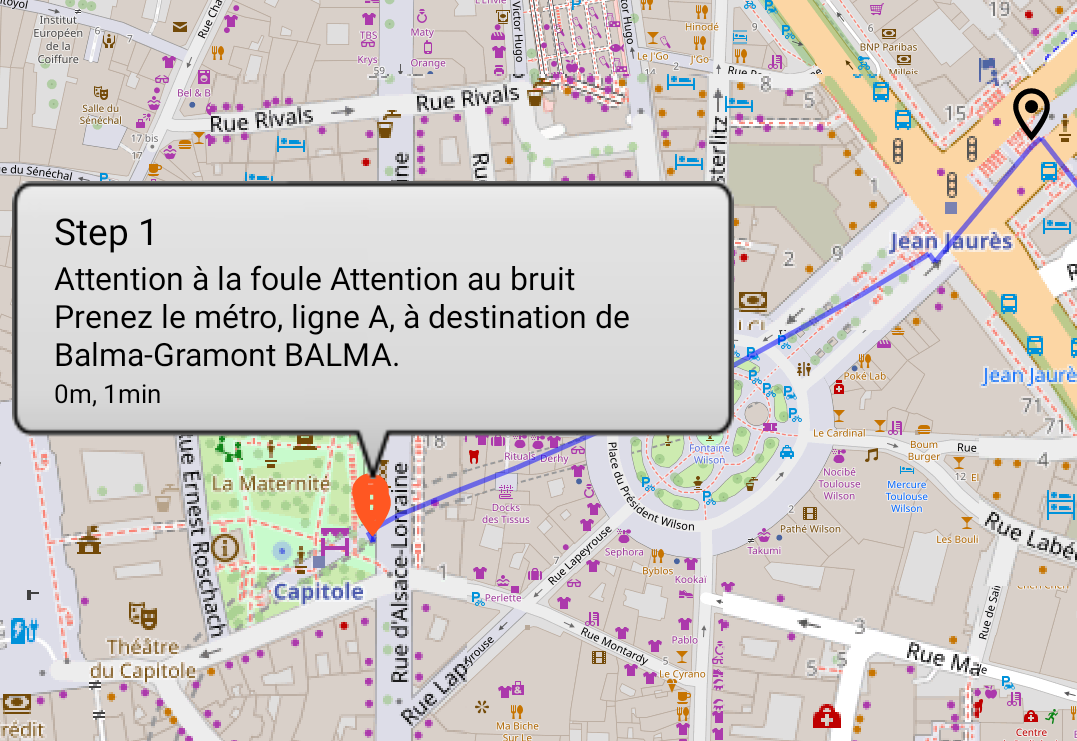
\includegraphics[scale=0.3]{img/step warning.png}
    \caption{Visualisation of a warning step}
    \label{fig:WarningStep}
\end{figure}

Finally, we conceived the journey planner as simply as possible, to not give too much information at the same time to the user and remove any uncertainty. The Tisseo API usually returns different possible paths to travel between destinations, but our application chooses the best out of all the available options and returns only one path to the user. The Tisseo API also allows our app to line up with public transport schedules, and this information can be relayed to the user so that they know how long they will stay at one location.
